% Created by tikzDevice version 0.10.1 on 2016-08-02 18:36:23
% !TEX encoding = UTF-8 Unicode
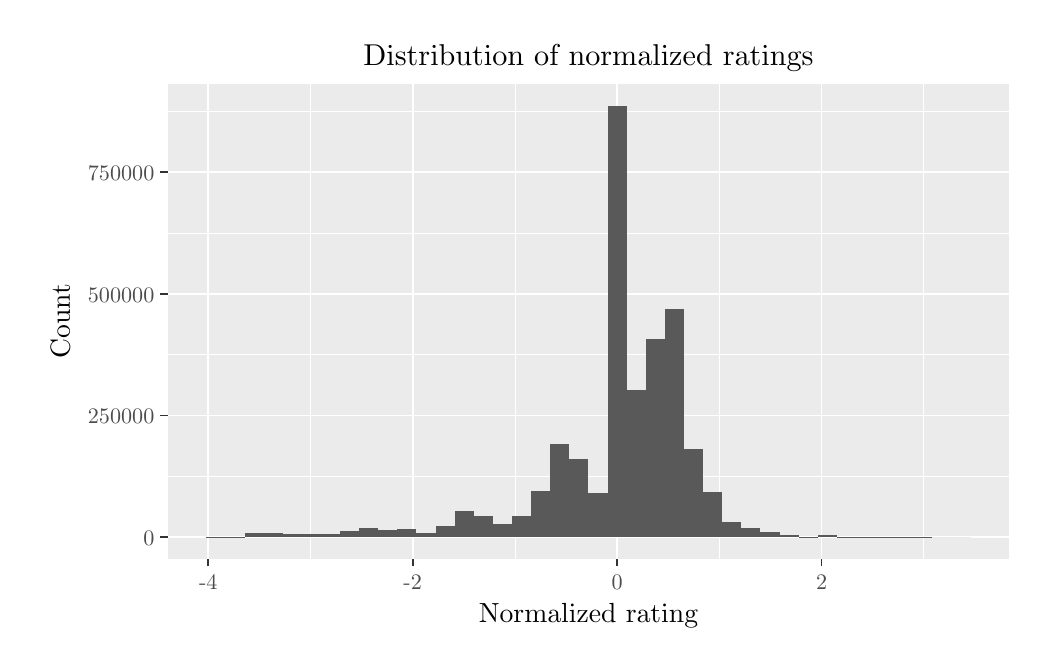
\begin{tikzpicture}[x=1pt,y=1pt]
\definecolor{fillColor}{RGB}{255,255,255}
\path[use as bounding box,fill=fillColor,fill opacity=0.00] (0,0) rectangle (360.07,222.54);
\begin{scope}
\path[clip] (  0.00,  0.00) rectangle (360.07,222.54);
\definecolor{drawColor}{RGB}{255,255,255}
\definecolor{fillColor}{RGB}{255,255,255}

\path[draw=drawColor,line width= 0.6pt,line join=round,line cap=round,fill=fillColor] (  0.00,  0.00) rectangle (360.07,222.54);
\end{scope}
\begin{scope}
\path[clip] ( 50.72, 30.62) rectangle (354.57,202.21);
\definecolor{fillColor}{gray}{0.92}

\path[fill=fillColor] ( 50.72, 30.62) rectangle (354.57,202.21);
\definecolor{drawColor}{RGB}{255,255,255}

\path[draw=drawColor,line width= 0.3pt,line join=round] ( 50.72, 60.40) --
	(354.57, 60.40);

\path[draw=drawColor,line width= 0.3pt,line join=round] ( 50.72,104.37) --
	(354.57,104.37);

\path[draw=drawColor,line width= 0.3pt,line join=round] ( 50.72,148.33) --
	(354.57,148.33);

\path[draw=drawColor,line width= 0.3pt,line join=round] ( 50.72,192.29) --
	(354.57,192.29);

\path[draw=drawColor,line width= 0.3pt,line join=round] (102.19, 30.62) --
	(102.19,202.21);

\path[draw=drawColor,line width= 0.3pt,line join=round] (176.07, 30.62) --
	(176.07,202.21);

\path[draw=drawColor,line width= 0.3pt,line join=round] (249.94, 30.62) --
	(249.94,202.21);

\path[draw=drawColor,line width= 0.3pt,line join=round] (323.82, 30.62) --
	(323.82,202.21);

\path[draw=drawColor,line width= 0.6pt,line join=round] ( 50.72, 38.42) --
	(354.57, 38.42);

\path[draw=drawColor,line width= 0.6pt,line join=round] ( 50.72, 82.39) --
	(354.57, 82.39);

\path[draw=drawColor,line width= 0.6pt,line join=round] ( 50.72,126.35) --
	(354.57,126.35);

\path[draw=drawColor,line width= 0.6pt,line join=round] ( 50.72,170.31) --
	(354.57,170.31);

\path[draw=drawColor,line width= 0.6pt,line join=round] ( 65.26, 30.62) --
	( 65.26,202.21);

\path[draw=drawColor,line width= 0.6pt,line join=round] (139.13, 30.62) --
	(139.13,202.21);

\path[draw=drawColor,line width= 0.6pt,line join=round] (213.01, 30.62) --
	(213.01,202.21);

\path[draw=drawColor,line width= 0.6pt,line join=round] (286.88, 30.62) --
	(286.88,202.21);
\definecolor{fillColor}{gray}{0.35}

\path[fill=fillColor] ( 64.53, 38.42) rectangle ( 71.44, 38.44);

\path[fill=fillColor] ( 71.44, 38.42) rectangle ( 78.35, 38.67);

\path[fill=fillColor] ( 78.35, 38.42) rectangle ( 85.25, 40.09);

\path[fill=fillColor] ( 85.25, 38.42) rectangle ( 92.16, 40.07);

\path[fill=fillColor] ( 92.16, 38.42) rectangle ( 99.06, 39.54);

\path[fill=fillColor] ( 99.06, 38.42) rectangle (105.97, 39.45);

\path[fill=fillColor] (105.97, 38.42) rectangle (112.87, 39.41);

\path[fill=fillColor] (112.87, 38.42) rectangle (119.78, 40.49);

\path[fill=fillColor] (119.78, 38.42) rectangle (126.68, 41.79);

\path[fill=fillColor] (126.68, 38.42) rectangle (133.59, 41.05);

\path[fill=fillColor] (133.59, 38.42) rectangle (140.50, 41.29);

\path[fill=fillColor] (140.50, 38.42) rectangle (147.40, 40.11);

\path[fill=fillColor] (147.40, 38.42) rectangle (154.31, 42.40);

\path[fill=fillColor] (154.31, 38.42) rectangle (161.21, 48.01);

\path[fill=fillColor] (161.21, 38.42) rectangle (168.12, 46.17);

\path[fill=fillColor] (168.12, 38.42) rectangle (175.02, 43.34);

\path[fill=fillColor] (175.02, 38.42) rectangle (181.93, 46.09);

\path[fill=fillColor] (181.93, 38.42) rectangle (188.84, 55.10);

\path[fill=fillColor] (188.84, 38.42) rectangle (195.74, 72.23);

\path[fill=fillColor] (195.74, 38.42) rectangle (202.65, 66.56);

\path[fill=fillColor] (202.65, 38.42) rectangle (209.55, 54.50);

\path[fill=fillColor] (209.55, 38.42) rectangle (216.46,194.41);

\path[fill=fillColor] (216.46, 38.42) rectangle (223.36, 91.46);

\path[fill=fillColor] (223.36, 38.42) rectangle (230.27,110.16);

\path[fill=fillColor] (230.27, 38.42) rectangle (237.17,121.05);

\path[fill=fillColor] (237.17, 38.42) rectangle (244.08, 70.36);

\path[fill=fillColor] (244.08, 38.42) rectangle (250.99, 54.76);

\path[fill=fillColor] (250.99, 38.42) rectangle (257.89, 43.79);

\path[fill=fillColor] (257.89, 38.42) rectangle (264.80, 41.84);

\path[fill=fillColor] (264.80, 38.42) rectangle (271.70, 40.23);

\path[fill=fillColor] (271.70, 38.42) rectangle (278.61, 39.18);

\path[fill=fillColor] (278.61, 38.42) rectangle (285.51, 38.63);

\path[fill=fillColor] (285.51, 38.42) rectangle (292.42, 39.25);

\path[fill=fillColor] (292.42, 38.42) rectangle (299.33, 38.52);

\path[fill=fillColor] (299.33, 38.42) rectangle (306.23, 38.45);

\path[fill=fillColor] (306.23, 38.42) rectangle (313.14, 38.46);

\path[fill=fillColor] (313.14, 38.42) rectangle (320.04, 38.43);

\path[fill=fillColor] (320.04, 38.42) rectangle (326.95, 38.43);

\path[fill=fillColor] (326.95, 38.42) rectangle (333.85, 38.42);

\path[fill=fillColor] (333.85, 38.42) rectangle (340.76, 38.42);
\end{scope}
\begin{scope}
\path[clip] (  0.00,  0.00) rectangle (360.07,222.54);
\definecolor{drawColor}{gray}{0.30}

\node[text=drawColor,anchor=base east,inner sep=0pt, outer sep=0pt, scale=  0.80] at ( 45.77, 35.41) {0};

\node[text=drawColor,anchor=base east,inner sep=0pt, outer sep=0pt, scale=  0.80] at ( 45.77, 79.37) {250000};

\node[text=drawColor,anchor=base east,inner sep=0pt, outer sep=0pt, scale=  0.80] at ( 45.77,123.33) {500000};

\node[text=drawColor,anchor=base east,inner sep=0pt, outer sep=0pt, scale=  0.80] at ( 45.77,167.29) {750000};
\end{scope}
\begin{scope}
\path[clip] (  0.00,  0.00) rectangle (360.07,222.54);
\definecolor{drawColor}{gray}{0.20}

\path[draw=drawColor,line width= 0.6pt,line join=round] ( 47.97, 38.42) --
	( 50.72, 38.42);

\path[draw=drawColor,line width= 0.6pt,line join=round] ( 47.97, 82.39) --
	( 50.72, 82.39);

\path[draw=drawColor,line width= 0.6pt,line join=round] ( 47.97,126.35) --
	( 50.72,126.35);

\path[draw=drawColor,line width= 0.6pt,line join=round] ( 47.97,170.31) --
	( 50.72,170.31);
\end{scope}
\begin{scope}
\path[clip] (  0.00,  0.00) rectangle (360.07,222.54);
\definecolor{drawColor}{gray}{0.20}

\path[draw=drawColor,line width= 0.6pt,line join=round] ( 65.26, 27.87) --
	( 65.26, 30.62);

\path[draw=drawColor,line width= 0.6pt,line join=round] (139.13, 27.87) --
	(139.13, 30.62);

\path[draw=drawColor,line width= 0.6pt,line join=round] (213.01, 27.87) --
	(213.01, 30.62);

\path[draw=drawColor,line width= 0.6pt,line join=round] (286.88, 27.87) --
	(286.88, 30.62);
\end{scope}
\begin{scope}
\path[clip] (  0.00,  0.00) rectangle (360.07,222.54);
\definecolor{drawColor}{gray}{0.30}

\node[text=drawColor,anchor=base,inner sep=0pt, outer sep=0pt, scale=  0.80] at ( 65.26, 19.64) {-4};

\node[text=drawColor,anchor=base,inner sep=0pt, outer sep=0pt, scale=  0.80] at (139.13, 19.64) {-2};

\node[text=drawColor,anchor=base,inner sep=0pt, outer sep=0pt, scale=  0.80] at (213.01, 19.64) {0};

\node[text=drawColor,anchor=base,inner sep=0pt, outer sep=0pt, scale=  0.80] at (286.88, 19.64) {2};
\end{scope}
\begin{scope}
\path[clip] (  0.00,  0.00) rectangle (360.07,222.54);
\definecolor{drawColor}{RGB}{0,0,0}

\node[text=drawColor,anchor=base,inner sep=0pt, outer sep=0pt, scale=  1.00] at (202.65,  7.70) {Normalized rating};
\end{scope}
\begin{scope}
\path[clip] (  0.00,  0.00) rectangle (360.07,222.54);
\definecolor{drawColor}{RGB}{0,0,0}

\node[text=drawColor,rotate= 90.00,anchor=base,inner sep=0pt, outer sep=0pt, scale=  1.00] at ( 15.24,116.42) {Count};
\end{scope}
\begin{scope}
\path[clip] (  0.00,  0.00) rectangle (360.07,222.54);
\definecolor{drawColor}{RGB}{0,0,0}

\node[text=drawColor,anchor=base,inner sep=0pt, outer sep=0pt, scale=  1.09] at (202.65,208.81) {Distribution of normalized ratings};
\end{scope}
\end{tikzpicture}
